\chapter{Incoherency} \label{chap:Incoherency}

In this chapter the blending operator is analyzed in greater detail. Then a measure for incoherency will be introduced. Finally, it will be discussed how deblending is influenced by incoherency and the so called maximum firing time delay.

\section{Analysis of the Blending Matrix} \label{sec:BlendingMatrix}

In order to optimize the blended acquisition design, one must understand the properties of the blending matrix, $\mathbf{\Gamma}$, and its influence on the deblending performance.

The blending matrix, $\mathbf{\Gamma}$, determines the pseudo-deblended data,

\begin{equation}
	\mathbf{P}_{ps} = \mathbf{P \Gamma \Gamma}^H,
	\label{eq:Ch-Theory-Pseudo-Deblended-Data}
\end{equation}

which are a superposition of the unblended data, $\mathbf{P}$, and the blending noise, $\mathbf{N}$,

\begin{equation}
	\mathbf{P}_{ps} = \mathbf{P} + \mathbf{N} = \mathbf{P I} + \mathbf{P} \; (\mathbf{\Gamma \Gamma}^H - \mathbf{I}).
	\label{eq:Ch-Theory-PseudoSuperposition}
\end{equation}

The more incoherent the blending noise, $\mathbf{N}$, the better it can be removed by noise filters.

In the following the effect of the blending matrix, $\mathbf{\Gamma}$, on the pseudo-deblended data, $\mathbf{P}_{ps}$, is analyzed. For simplicity, it is assumed that all shots are equal in strength and fire the same signature into the earth. It is also assumed that each shot is fired only once, unlike e.g. the shot repetition case \citep{Sixue}. This means that the blending matrix, $\mathbf{\Gamma}$, only contains phase shift terms, $\mathrm{e}^{-j \omega \Delta t}$, or zeros.

Each row of $\mathbf{\Gamma}$ represents a shot $k$, and each column of $\mathbf{\Gamma}^H$ represents a shot $l$ with a complex conjugated phase term (see Figure \ref{fig:Ch-Theory-GGH}). Hence, each element $g_{kl}$ of the matrix $\mathbf{\Gamma \Gamma}^H$ is the dot product between the $k^{th}$ shot and the complex conjugate of the $l^{th}$ shot.

\begin{figure}
	\centering
	\includegraphics[width = \textwidth]{Plots/GGH_v2}
	\caption{Illustration of the matrix product, $\mathbf{\Gamma \Gamma}^H$. In this notation $\Delta t_k$ refers to the phase shift of the shot $k$, and $\Delta t_{kl}$ refers to the phase shift between the shots $k$ and $l$, $\Delta t_{kl} = \Delta t_k - \Delta t_l$.}
	\label{fig:Ch-Theory-GGH}
\end{figure}

Consequently, an element $g_{kl}$ of the matrix product, $\mathbf{\Gamma \Gamma}^H$, represents the overlap of the shots $k$ and $l$ for all experiments. The main diagonal of $\mathbf{\Gamma \Gamma}^H$ refers to the overlap of each shot with itself, which of course is perfect and therefore equal to 1. The off diagonal elements of $\mathbf{\Gamma \Gamma}^H$ are either 0 if the associated shots do not overlap, or contain a phase shift, $\mathrm{e}^{\, -j \omega \Delta t_{kl}}$.

\subsection*{Temporal incoherency}

In the following the term "sub-diagonal" will be used to refer to an arbitrary diagonal of the matrix $\mathbf{\Gamma \Gamma}^H$. For example, the $d^{th}$ sub-diagonal includes all the matrix elements $g_{ij}$, which fulfill the condition; $j -i = d$.

In equation \ref{eq:Ch-Theory-PseudoSuperposition} the main diagonal elements of $\mathbf{\Gamma \Gamma}^H$ copy the data matrix, $\mathbf{P}$, while the off-diagonal elements create the blending noise, $\mathbf{N}$. In case of constant firing time delays the elements along a sub-diagonal $d$ all have the same phase. This means that the sub-diagonal elements will shift the columns of the data matrix and apply a constant phase shift to each of them resulting in the pseudo-deblended receiver gather shown in Figure \ref{fig:Ch-Theory-PseudoCRG-CoherentDelay}. Instead if firing times are not constant but random the elements $g_{ij}$ along a sub-diagonal $d$ will have different phases. Consequently, they will shift the columns of the data matrix and distort the phase of each column (see Figure \ref{fig:Ch-Theory-PseudoCRG-IncoherentDelay}). 

Figure \ref{fig:Ch-Theory-PseudoCRG-FK-CoherentDelay} and \ref{fig:Ch-Theory-PseudoCRG-FK-IncoherentDelay} display the $f$-$k$-spectra of the pseudo-blended data for constant firing time delays and random firing time delays respectively. In the case of constant firing time delays all of the energy maps in the signal cone. In the case of random firing time delays a significant part of the energy maps outside of the signal cone. From Figure \ref{fig:Ch-Theory-PseudoCRG-FK-CoherentDelay} and \ref{fig:Ch-Theory-PseudoCRG-FK-IncoherentDelay} it is clear that the coherency constraint presented in section \ref{sec:IterBlenNoiseEst} cannot work with constant firing time delays, but needs the random firing time delays. 

In this thesis the random firing time delays along a sub-diagonal are referred to as temporal incoherency.  

\begin{figure}
	\centering
	\begin{subfigure}[b]{0.3\textwidth}
		\centering
		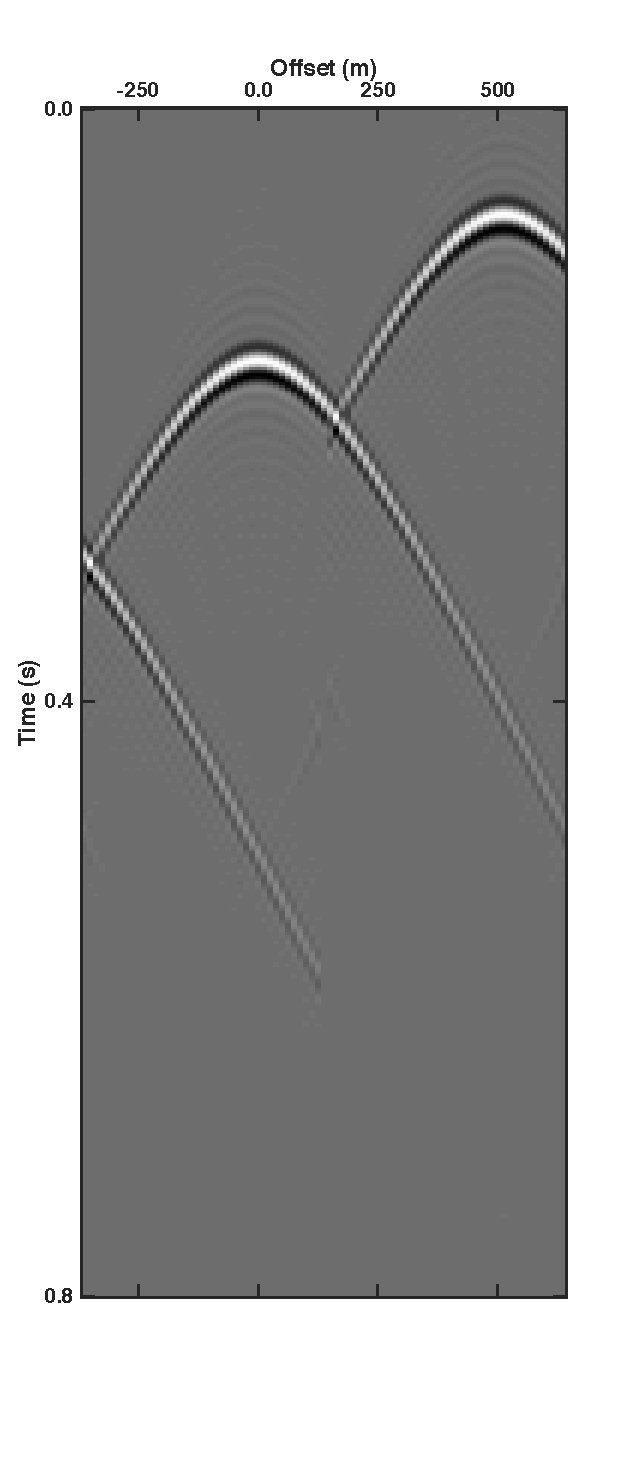
\includegraphics[width = \textwidth]{Plots/Mahdad/25iter/TimeDelay/Pseudo-DeblendedCRG_rec30_coh}
		\caption{}
		\label{fig:Ch-Theory-PseudoCRG-CoherentDelay}
	\end{subfigure}
	%
	\centering
	\begin{subfigure}[b]{0.3\textwidth}
		\centering
		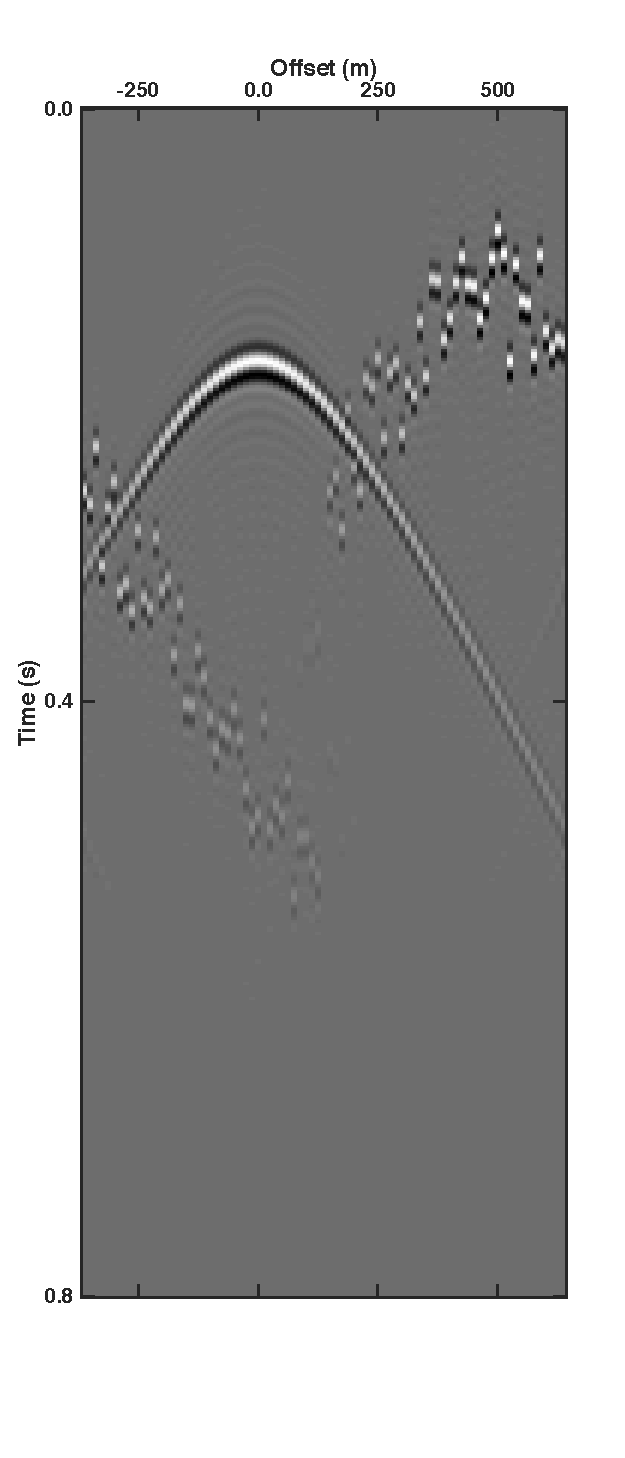
\includegraphics[width = \textwidth]{Plots/Mahdad/25iter/TimeDelay/Pseudo-DeblendedCRG_rec30}
		\caption{}
		\label{fig:Ch-Theory-PseudoCRG-IncoherentDelay}
	\end{subfigure}
	%
	\centering
	\begin{subfigure}[b]{0.3\textwidth}
	
		\centering
		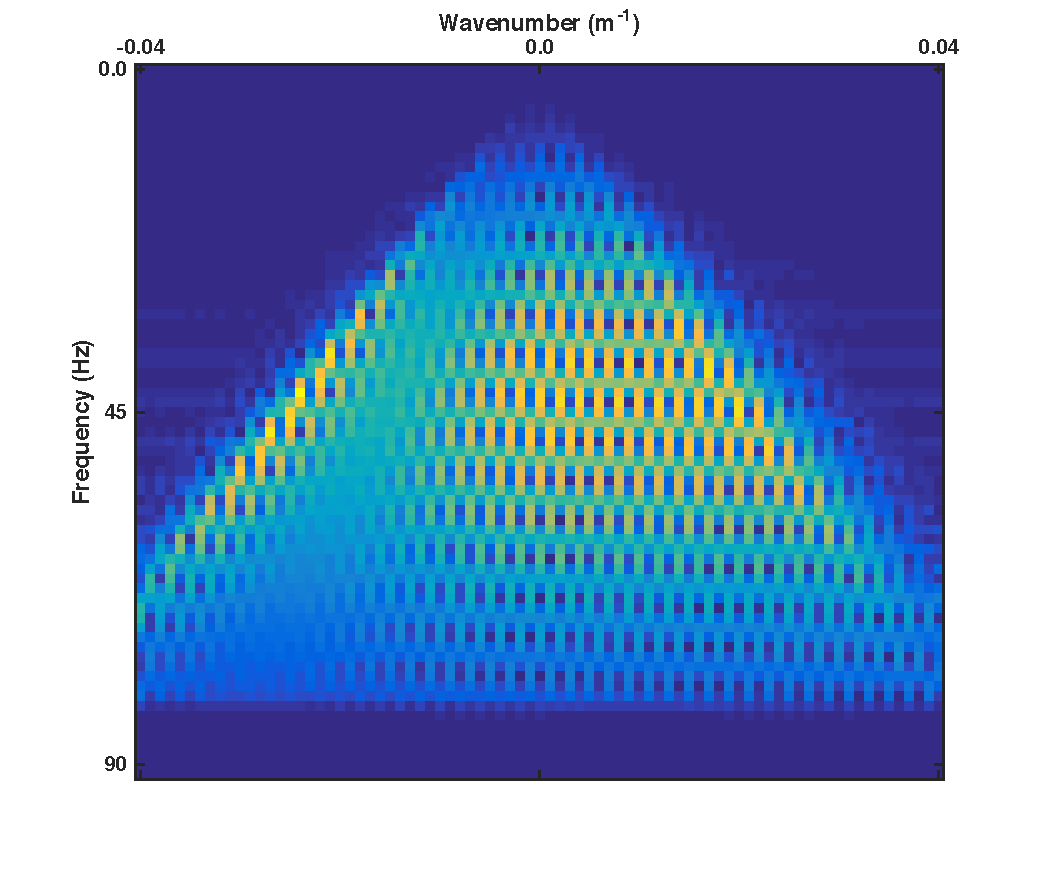
\includegraphics[width = \textwidth]{Plots/Mahdad/25iter/TimeDelay/FK-Pseudo-deblendedCRG_rec30_coh}
		\caption{}
		\label{fig:Ch-Theory-PseudoCRG-FK-CoherentDelay}
		
		\par\bigskip
		
		\centering
		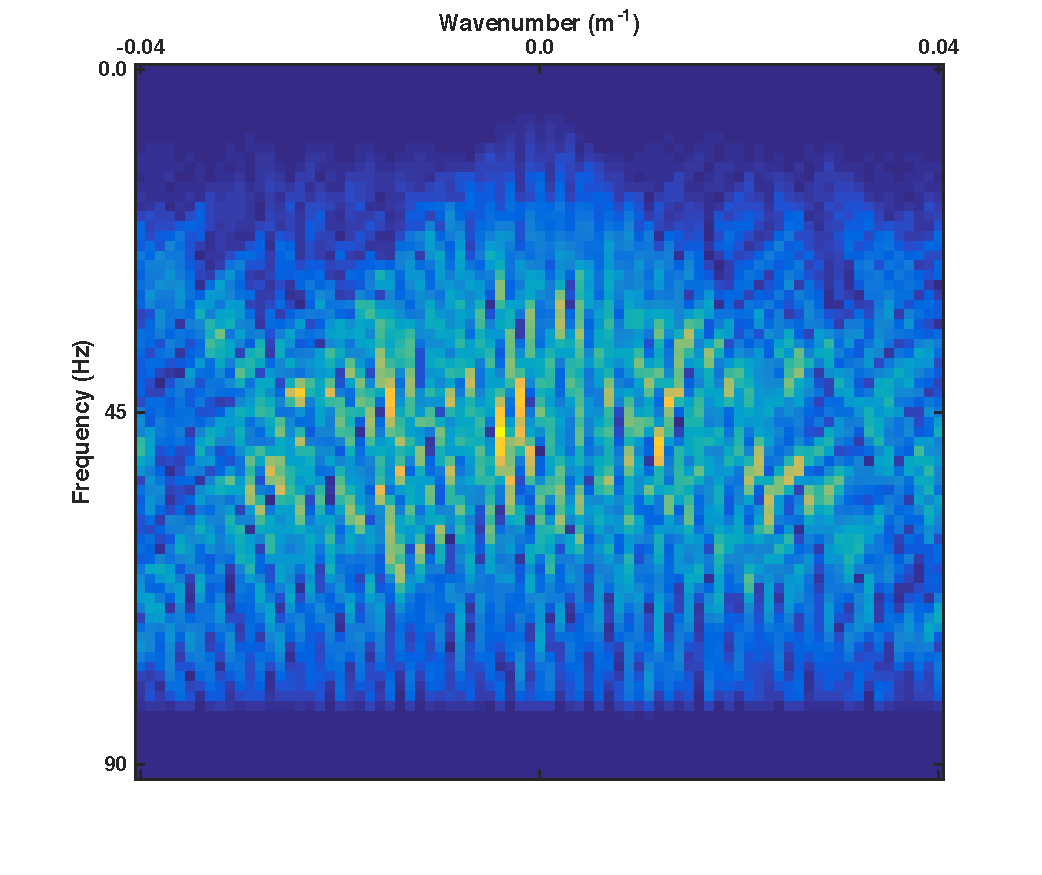
\includegraphics[width = \textwidth]{Plots/Mahdad/25iter/TimeDelay/FK-Pseudo-deblendedCRG_rec30}
		\caption{}
		\label{fig:Ch-Theory-PseudoCRG-FK-IncoherentDelay}
		
	\end{subfigure}
	
	\caption{Comparison of the pseudo-deblended receiver gather for (a) constant firing time delays of \SI{100}{\milli\second}, and (b) random firing time delays between \SI{0}{\milli\second} and \SI{100}{\milli\second}. (c) and (d) show the $f$-$k$-spectra of (a) and (b) respectively.}
	\label{fig:Ch-Theory-PseudoCRG-IncoherencyEffect}

\end{figure}

\begin{figure}
	\centering
	\includegraphics[width=\textwidth]{Plots/GGH_x_v2}
	\caption{The blending matrix, $\mathbf{\Gamma}$, is obtained by interchanging the $3^{rd}$ and $4^{th}$ row of the blending matrix in Figure \ref{fig:Ch-Theory-GGH}. In acquisition this is equivalent to moving shot 3 to experiment 2, and shot 4 to experiment 1. A random permutation of the rows of the blending matrix spreads the off-diagonal elements of the matrix product, $\mathbf{\Gamma\Gamma}^H$. The elements are not assembled on the sub-diagonals anymore.}
	\label{fig:Ch-Theory-GGHx}
\end{figure}

\begin{comment}
In order to generate incoherent source interference, $\mathbf{N}$, it is therefore favorable if the elements $a_{ik}$ of each lower or upper diagonal are out of phase. For example, considering the $n^{th}$ upper or lower diagonal of the matrix $\mathbf{\Gamma \Gamma}^H$ this observation translates to the acquisition as follows: All source pairs, which are $n$ sources apart from each other, must be fired incoherently. The incoherent firing is realized by delaying blended sources with a random time delay.
\end{comment}


\subsection*{Spatial incoherency}

Of course, the degree of incoherency of the blending noise, $\mathbf{N}$, also depends on whether the shot positions of shots blended in an experiment are selected randomly, or in a spatially coherent pattern. For example, one expects the blending noise to be more incoherent if in each experiment randomly selected shot positions are blended as in Figure \ref{fig:Ch-Theory-GGHx}, than if in each experiment adjacent shot positions are blended as in Figure \ref{fig:Ch-Theory-GGH}, because the interfering shots are spread over the sub-diagonals in Figure \ref{fig:Ch-Theory-GGHx}.

In this thesis selecting random shots for an experiment is referred to as spatial incoherency.

Although examples of spatial incoherency are shown in this chapter, it has to be noted that to blend shots in a spatially incoherent fashion is not very practical in 2D acquisition. However, in chapter \ref{chap:MahdadMethod3d} it will be shown that for 3D blending spatial incoherency becomes feasible.


\begin{comment}

In terms of the blending matrix $\mathbf{\Gamma}$ a spatially incoherent firing pattern means that the rows, i.e. the sources, are shuffled randomly. As a consequence the off-diagonal elements of the matrix product $\mathbf{\Gamma \Gamma}^H$ are reordered randomly. This shuffling process can help to further distort the phase of the interfering sources. However, if the maximum allowed time delay between blended sources is aready large the spatially incoherent blending pattern will not increase the incoherency of the interfering sources.   

In practice, the maximum allowed firing time delay is limited by the available acquisition time. The spatial distribution of blended sources is constraint by the acquisition design.
	
\end{comment}


\FloatBarrier

\section{Effect of Incoherency} \label{sec:Effect-of-Incoherency}

This section aims to analyze how strongly the deblending result depends on the incoherency of the blended acquisition. For this purpose a measure of incoherency and deblending quality will be introduced. Then, the possibilities of creating an incoherent blending pattern are presented.

\subsection*{Incoherency Measure}

\todo[inline]{Move this sentence to the introduction (literature). You might also want to mention the work of the Greek guy Apostolos.\\
In this thesis only the incoherency of the acquisition design is considered. Thus, the blending matrix, $\Gamma$, or more precisely the product $\mathbf{\Gamma \Gamma}^H$ determines the incoherency.}

%A measure of incoherency will be introduced in order to analyze the importance of an incoherent blending pattern quantitatively.

In section \ref{sec:BlendingMatrix} it was shown that for an incoherent blending pattern the elements, $\mathrm{e}^{-j \omega \Delta t_{kl}}$, along a sub-diagonal of the matrix product, $\mathbf{\Gamma \Gamma}^H$, should be out of phase. Therefore, the phase variability of the sub-diagonal elements will be used to quantify incoherency. 

\begin{figure}
	\centering
	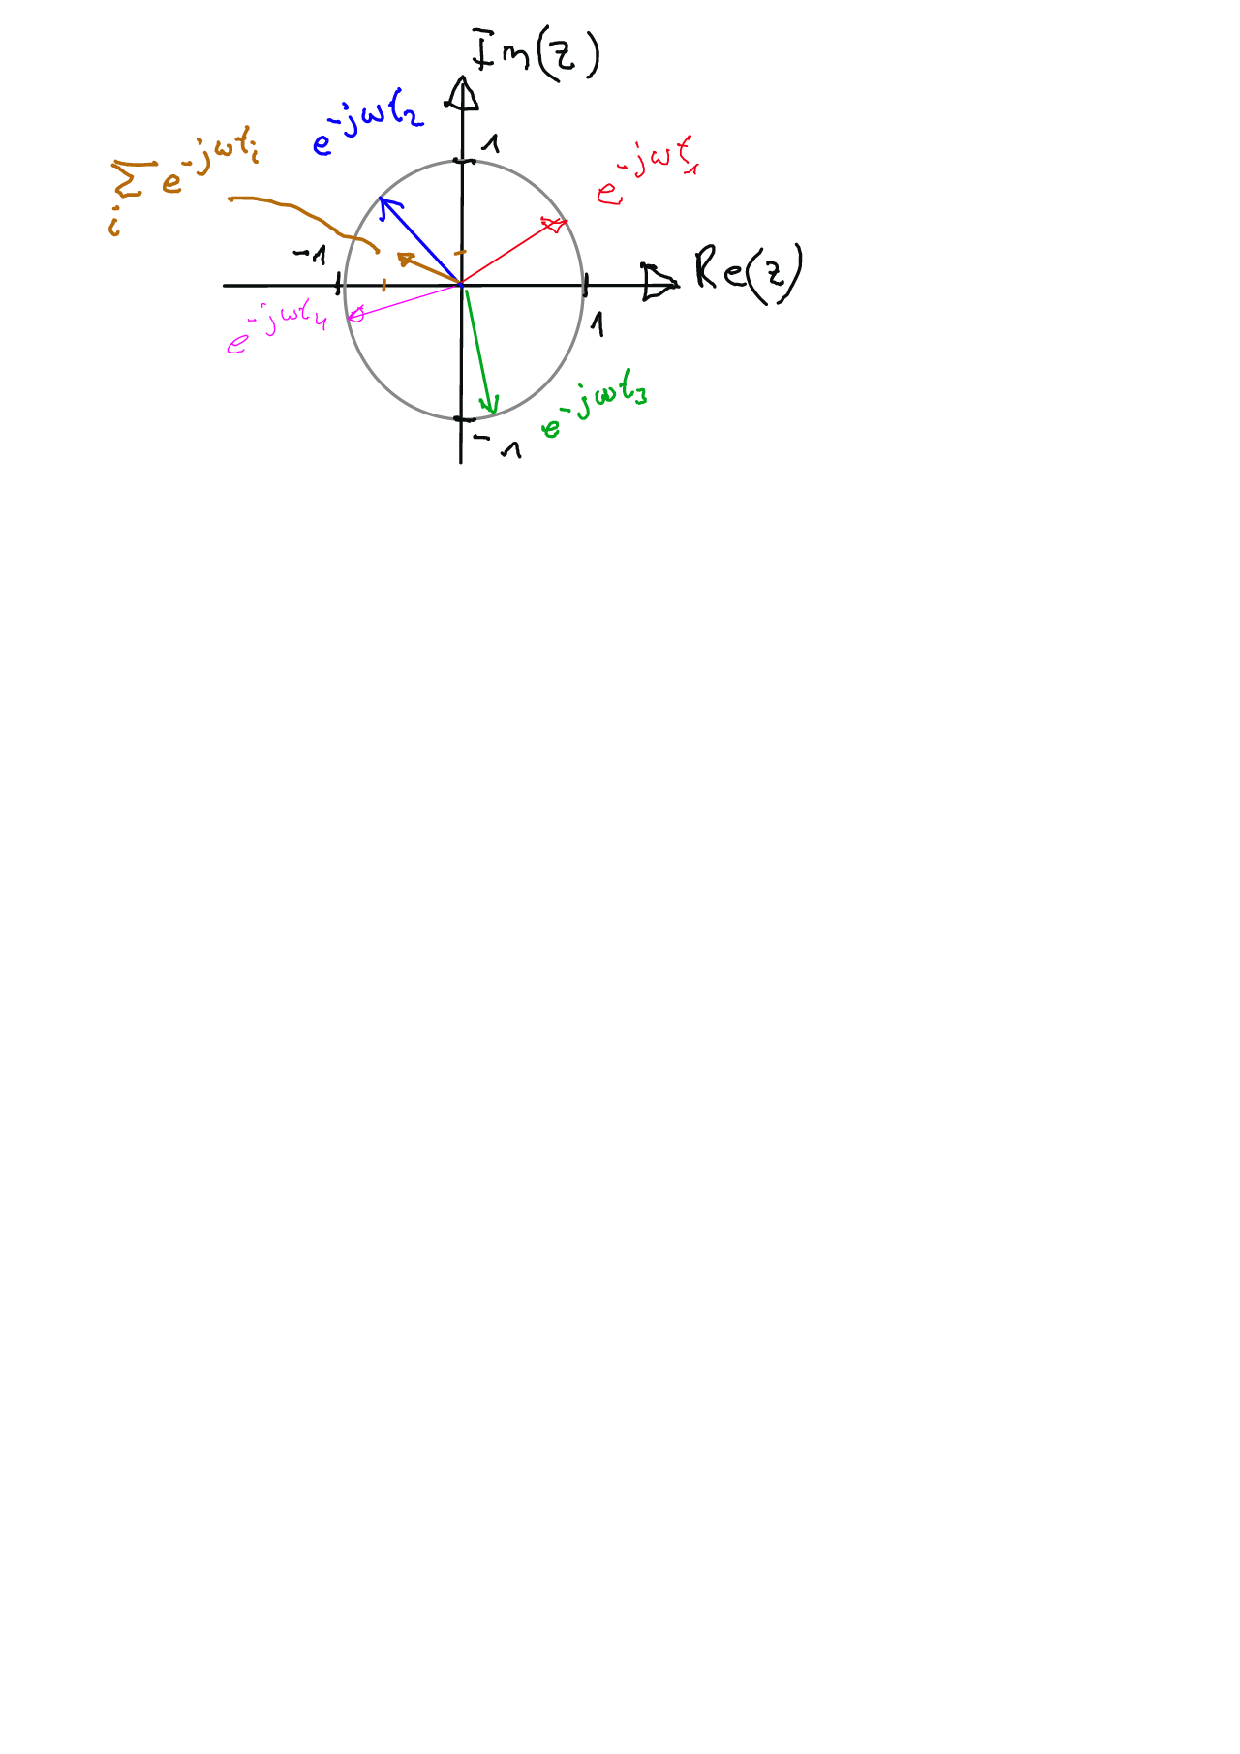
\includegraphics[width = 0.5\textwidth]{Plots/complex-circle}
	\caption{Illustration of the sub-diagonal elements in the complex number plane. The elements have unit length and variable phase. The absolute value of their sum depends on the phase coherency of the elements.}
	\label{fig:Ch-Results-complex-circle}
\end{figure}

The sub-diagonal elements, $\mathrm{e}^{-j \omega \Delta t_{kl}}$, map in the complex plane on a circle with radius 1 (see Figure \ref{fig:Ch-Results-complex-circle}). Thus, the sum of the elements along the $d^{th}$ sub-diagonal can be constructive or destructive, depending on the phase variability. The absolute value of this sum, $S(d,\omega)$, measures the incoherency of the $d^{th}$ sub-diagonal for the frequency component, $\omega$;

\begin{equation}
	S(d,\omega) = \left| \sum_{j-i=d} \mathbf{\Gamma \Gamma}^H_{ij} (\omega) \right|.
	\label{eq:Ch-Results-incoherency-diagsum}	
\end{equation} 

For example, if all sub-diagonal elements are in phase the absolute value of their sum, $S(d,\omega)$, is maximized. Instead, in case of an incoherent blending pattern $S(d,\omega)$ is small for all sub-diagonals $d$, except for the main diagonal ($d = 0$).  

Next, $S(d,\omega)$ is summed over all frequency components, $\omega$. Each element of the resulting vector $S(d)$ is squared in order to relate it to energy. Finally, the incoherency, $\mu$, is quantified by the ratio of the main diagonal result and the sum of all sub-diagonal results;

\begin{equation}
	\mu = \frac{\left( \; \sum_{\omega}S(d=0,\omega) \; \right)^2}{\sum_{d = 1-Ns}^{Ns-1} \left(\left( \; \sum_{\omega}S(d,\omega) \; \right)^2\right)}
	\label{eq:Ch-Results-incoherency}
\end{equation}

Note that $N_s$ is the number of sources, i.e. the matrix $\mathbf{\Gamma \Gamma}^H$ has $N_s$ rows and columns. Equation \ref{eq:Ch-Results-incoherency} implies that the incoherency value can vary between 0 (perfectly coherent) and 1 (perfectly incoherent).

For example, consider the two blending matrices, $\mathbf{\Gamma}_{coh}$ and $\mathbf{\Gamma}_{ran}$, which produce the pseudo-deblended receiver gathers in Figure \ref{fig:Ch-Theory-PseudoCRG-CoherentDelay} and \ref{fig:Ch-Theory-PseudoCRG-IncoherentDelay} respectively. The blending matrix, $\mathbf{\Gamma}_{coh}$, uses coherent firing time delays, while the blending matrix, $\mathbf{\Gamma}_{ran}$, uses random firing time delays. Figure \ref{fig:Ch-Incoherency-Coh-vs-Ran-Diag} shows $S(d,\omega)$ for both blending matrices for the frequency slice $f=\SI{25}{\hertz}$. One observes that the coherent blending matrix, $\mathbf{\Gamma}_{coh}$, results in a less spike-like $S(d,\omega)$ function than the incoherent blending matrix, $\mathbf{\Gamma}_{ran}$.

\begin{figure}
	
	\centering
	\begin{subfigure}[b]{0.45\textwidth}
	\centering
	\includegraphics[width = \textwidth]{Plots/DiagonalSums/diagsums_coherent}	
	\caption{}
	\label{fig:Ch-Incoherency-CoherentDiag}	
	\end{subfigure}
	%
	\centering
	\begin{subfigure}[b]{0.45\textwidth}
	\centering
	\includegraphics[width = \textwidth]{Plots/DiagonalSums/diagsums_random}	
	\caption{}
	\label{fig:Ch-Incoherency-RandomDiag}	
	\end{subfigure}
	
	\caption{Illustration of the absolute sub-diagonal sums, $S(d,\omega)$, for the frequency slice $f=\SI{25}{\hertz}$. (a) refers to the blending matrix $\mathbf{\Gamma}_{coh}$ with coherent firing time delays.  $S(d,\omega)$ is less spike-like and yields an incoherency value of $\mu_a = \SI{67}{\percent}$. (b) refers to the blending matrix $\mathbf{\Gamma}_{ran}$ with random firing time delays. $S(d,\omega)$ is  close to a spike and yields an incoherency value of $\mu_b = \SI{98}{\percent}$.}
	\label{fig:Ch-Incoherency-Coh-vs-Ran-Diag}
	
\end{figure}


\subsection*{Deblending Performance Measure}

The following data examples are synthetic data, i.e. the unblended data are known. Therefore, the deblending performance can be measured with the quality factor, $Q$, which is defined by \citet{IbrahimQuality} as the ratio of unblended data, $\mathbf{P}$, and the misfit between unblended data, $\mathbf{P}$, and deblended data, \textbf{\^{P}};

\begin{equation}
	Q = 10 \cdot \mathrm{log_{10}} \left( \frac{\left|\left|\mathbf{P}\right|\right| _2 ^2}{\left|\left|\mathbf{P - \hat{P}}\right|\right| _2 ^2} \right) \;.	
\end{equation}


\subsection*{Incoherent Blending Patterns}

Based on the blending matrices in Figure \ref{fig:Ch-Theory-GGH} and \ref{fig:Ch-Theory-GGHx} there are three possibilities to blend the shots incoherently. First, the phase terms along the sub-diagonals can be randomly varied, i.e. the shots are blended with random firing time delays (temporal incoherency). Second, the rows of the blending matrix can be randomly permuted, i.e. one randomly selects shots for each experiment (spatial incoherency). Third, temporal and spatial incoherency can be combined (mixed incoherency), i.e. randomly selected shots are blended with random firing time delays.



\section{Results}

In the following the 3 blending patterns presented in section \ref{sec:Effect-of-Incoherency} will be applied to a synthetic data set. The data are a common receiver gather with 21 shots (see Figure \ref{fig:Ch-Results-Unbl-inline10}), which are blended in 3 experiments with 7 shots per experiment. Next, the data are deblended with the deblending algorithm of section \ref{sec:MahdadMethod}. 

The deblending results are shown in Figure \ref{fig:Ch-Results-Debl-x-inline}. The results suggest that only spatial incoherency is not sufficient to deblend the data (see Figure \ref{fig:Ch-Results-Debl-inline10-x}). By introducing random firing time delays the deblended data improve significantly as shown in Figure \ref{fig:Ch-Results-Debl-inline10-t}. A combination of both spatial and temporal incoherency enhances the deblended data further (see Figure \ref{fig:Ch-Results-Debl-inline10-xt}).


\begin{figure}
	\centering
	\begin{subfigure}[t]{0.24\textwidth}
		\centering
		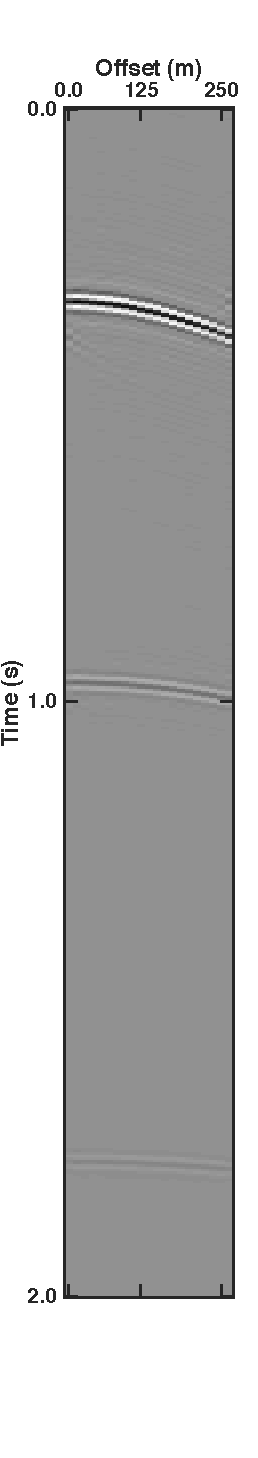
\includegraphics[height = 0.38\textheight]{Plots/BlendingPatterns/Unblended_xline10}
		\caption{}
		\label{fig:Ch-Results-Unbl-inline10}
	\end{subfigure}
	%	
	\centering
	\begin{subfigure}[t]{0.24\textwidth}
		\centering
		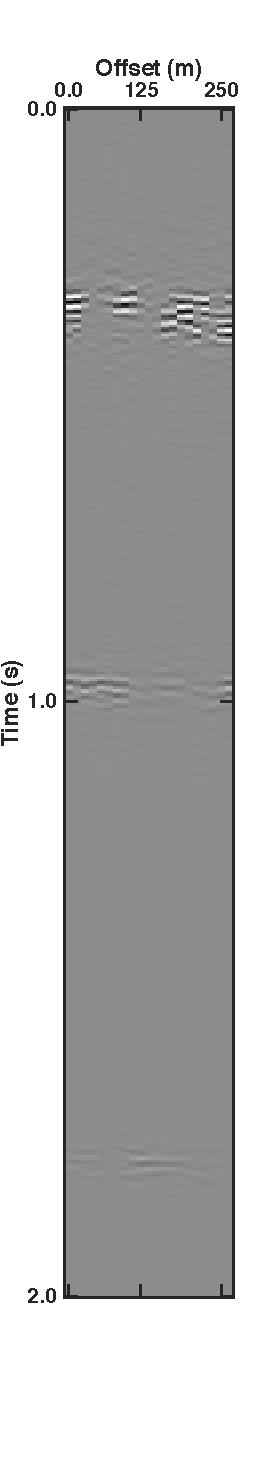
\includegraphics[height = 0.38\textheight]{Plots/BlendingPatterns/Deblended_xline10x}
		\caption{}
		\label{fig:Ch-Results-Debl-inline10-x}
	\end{subfigure}
	%
	\centering
	\begin{subfigure}[t]{0.24\textwidth}
		\centering
		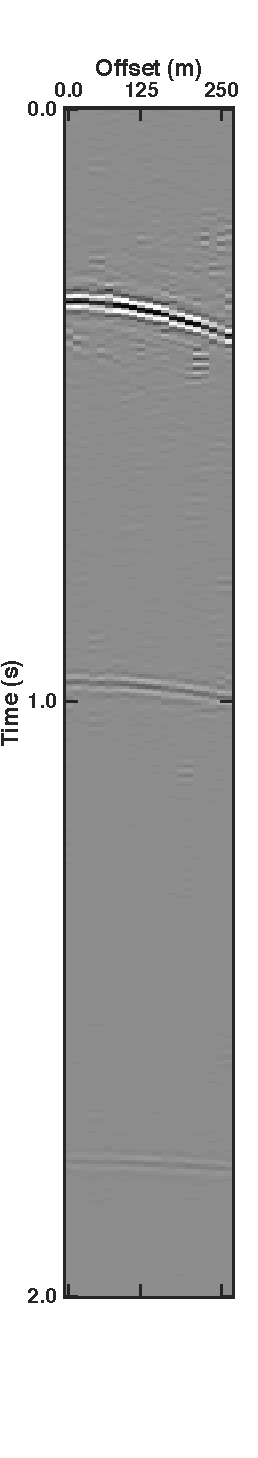
\includegraphics[height = 0.38\textheight]{Plots/BlendingPatterns/Deblended_xline10t}
		\caption{}
		\label{fig:Ch-Results-Debl-inline10-t}
	\end{subfigure}
	%
	\centering
	\begin{subfigure}[t]{0.24\textwidth}
		\centering
		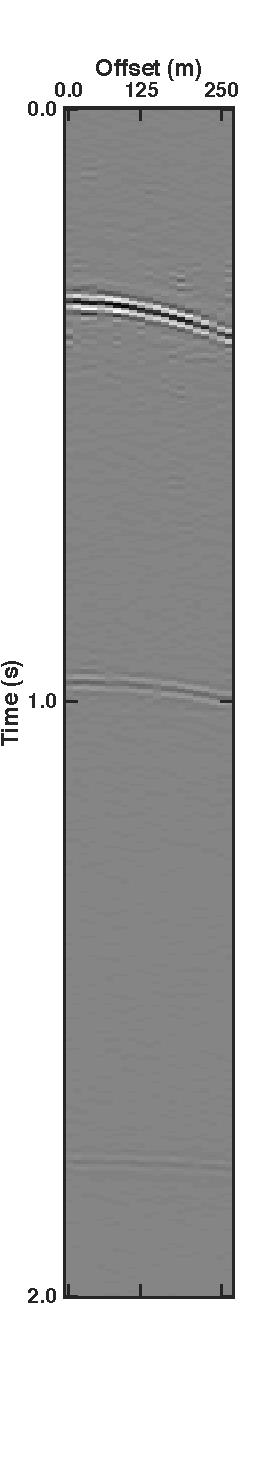
\includegraphics[height = 0.38\textheight]{Plots/BlendingPatterns/Deblended_xline10xt}
		\caption{}
		\label{fig:Ch-Results-Debl-inline10-xt}
	\end{subfigure}
	
	\caption{(a) shows an synthetic unblended common receiver gather. The data are blended with a (b) spatially incoherent, (c) temporally incoherent, and (d) mixed incoherent blending pattern. The respective deblending results are shown in (b) to (d).}
	\label{fig:Ch-Results-Debl-x-inline}

\end{figure}


Next, a quantitative analysis of the effect of incoherency, $\mu$, on the deblending quality, $Q$, is performed. For this purpose blending matrices with incoherencies between \SI{5}{\percent} and \SI{100}{\percent} are generated. The synthetic data are blended and deblended with these blending matrices. Figure \ref{fig:Ch-Results-QvsMu} illustrates the resulting quality factors as a function of the incoherency. 

\begin{figure}
	\centering
	\includegraphics[width = 0.6\textwidth]{Plots/Incoherency/Q-vs-Mu}
	\caption{Quality factor, $Q$, as a function of the incoherency, $\mu$. The deblending results with quality factors above 5 look acceptable.}
	\label{fig:Ch-Results-QvsMu}
\end{figure}

This result demonstrates that an incoherent blending pattern is inevitable for a good deblending result. However, only within a small range of incoherencies the deblending quality is sensitive to incoherency. Therefore, incoherency by its own is not a suitable parameter to adjust the desired quality factor.


\section{Effect of Maximum Firing Time Delay}

Another control factor of the deblending quality is the maximum firing time delay. In an extreme case of infinitely long maximum firing time delay the acquisition is not blended any more, and the deblending result is perfect. Hence, increasing maximum firing time delays are expected to enhance the deblending quality, but they require more acquisition time.



\section{Results}

The three suggested blending patterns namely temporal, spatial and mixed incoherency are applied to synthetic data with varying maximum firing time delays. 

Figure \ref{fig:Ch-Results-QualityFactors} shows the quality factors for the three blending patterns as a function of maximum firing time delay. Note that for a fixed maximum firing time delay and a specific blending pattern the firing time delays are generated with a random number generator. Consequently, the resulting quality factor varies depending on the variation of the random number series. For this reason several blending matrices are generated for each maximum firing time delay and each blending pattern. The resulting quality factors are averaged.

According to Figure \ref{fig:Ch-Results-QualityFactors} the spatially incoherent blending pattern yields a constant deblending quality independent of the maximum firing time delay. This is expected because it blends the sources without time delay. The deblending quality provided by the other two blending patterns continuously enhances with increasing maximum firing time delay. The difference in deblending quality between temporal and mixed blending patterns seems to be independent of the maximum firing time delay.

\begin{figure}
	\centering
	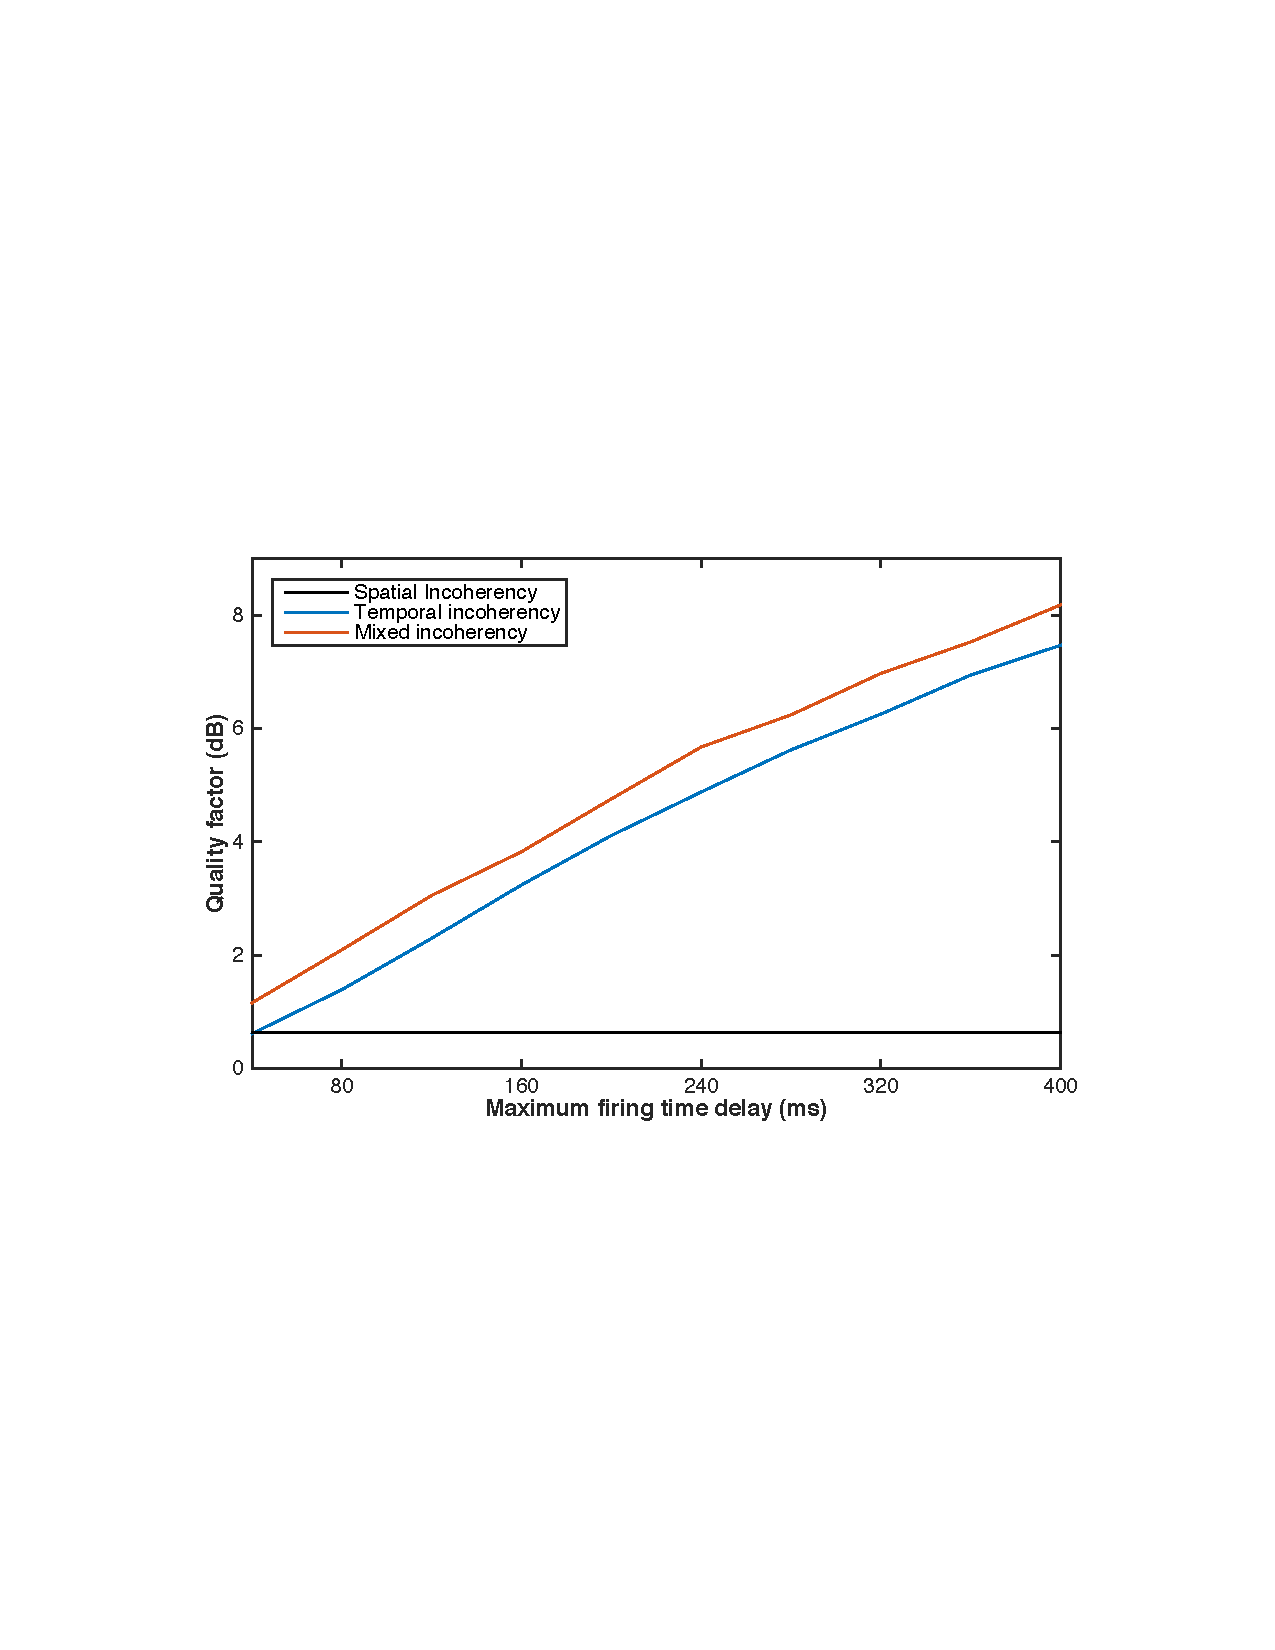
\includegraphics[width = 0.6\textwidth]{Plots/BlendingPatterns/quality_line_plot_avg}
	\caption{The 3 suggested blending patterns are simulated with maximum firing time delays between \SI{40}{\milli\second} and \SI{400}{\milli\second}. The quality factors are computed with respect to the unblended data and illustrated as a function of the maximum firing time delay.}
	\label{fig:Ch-Results-QualityFactors}
\end{figure}

\todo[inline]{For the conclusion/discussion of these results: \\ 
				Say that a high degree of incoherency is required for successful deblending, but it is not useful as a control factor of the deblending performance. Instead the maximum firing time delay allows to fine tune the quality factor and might be suitable to fine tune a trade off between deblending quality and acquisition time.\\
				One can also say that the  spatial incoherency performs poorly because its degree of incoherency is simply too low.}
			
			
				
\subsection*{Combination of Incoherency and Maximum Firing Time Delay}

In Figure \ref{fig:Ch-Results-QualityFactors} the quality factors are averaged for each maximum firing time delay and blending pattern. This means that for a given maximum firing time delay and blending pattern there are random firing time delays which yield better deblending results than other firing time delays.

In practice, the maximum firing time delay is given by the available acquisition time. For optimal deblending results the incoherency of the blending pattern should be maximized.

For example, consider again the two blending matrices, $\mathbf{\Gamma}_{coh}$ and $\mathbf{\Gamma}_{ran}$, which produced the pseudo-deblended receiver gathers in Figure \ref{fig:Ch-Theory-PseudoCRG-CoherentDelay} and \ref{fig:Ch-Theory-PseudoCRG-IncoherentDelay} respectively. Both blending matrices use the same maximum firing time delay. However, their incoherency values differ because $\mathbf{\Gamma}_{coh}$ uses coherent firing time delays whereas $\mathbf{\Gamma}_{ran}$ uses random firing time delays. 

An effective blending matrix, $\mathbf{\Gamma}_{eff}$, is created by superimposing both blending matrices;

\begin{equation}
	\mathbf{\Gamma}_{eff} = a \cdot \mathbf{\Gamma}_{ran} + (1 - a) \cdot \mathbf{\Gamma}_{coh}, \; a \in [0,1].
	\label{eq:Ch-Incoherency-EffectiveG}
\end{equation}

\todo[inline]{superposition must be in the time domain!}

The maximum firing time delay of the effective blending matrix, $\mathbf{\Gamma}_{eff}$, is constant while the incoherency  varies with changing $a$. The resulting quality factors are shown as a function of the incoherency in Figure \ref{fig:Ch-Results-Quality-vs-Incoherency}.

\begin{figure}
	\centering
	\includegraphics[width = 0.6\textwidth]{Plots/BlendingPatterns/Mu-vs-Q}
	\caption{Deblending quality as a function of incoherency for a constant maximum firing time delay.}
	\label{fig:Ch-Results-Quality-vs-Incoherency}
\end{figure}




























